\chapter{Results}

The following chapter presents the results of our study on a selection of datasets. I begin by providing an overview of each dataset. Afterward, the results of multiple experiments that we conducted are presented, including a description of each experiment and the corresponding results. The aim is to showcase some findings and give insight into the process of utilizing NeRFs.

\begin{comment}

Experiments:
- Explore the impact of capturing
    - Capturing NeRFs in different ways
        - Walking, standing still, sparsely, densely, linearly, around an object
    - Capturing video, images, polycam
        - Better/worse quality with polycam or COLMAP
    - Capturing different kind of scenes
        - Bounded/Unbounded 
    - Capturing in different conditions
    - Capturing 
    
- Explore the impact of dataset size
    - Extract different amounts of images from the video ✅
        - Simulate driving by walking up and back a street multiple times ✅
    - How much data is required until COLMAP becomes a bottleneck

- Explore the impact of area-size
    - Remember to point out that area is poorly defined since scale is perspective relative, depending on the level of detail you want. ✅
    - Area must be defined for a certain scene type. E.g. street view, aerial view, unbounded in multiple directions, bounded in all directions

- Explore the impact of different methods
    - instant-npg, nerfacto, NeRF

Metrics
- Quantitative
    - PSNR, LPIPS, SSIM
- Qualitative
    - Compare images side-by-side



Research questions:
- To what extent does a good capture impact the result of a NeRF
- How much data is required until COLMAP becomes a bottleneck?
- What is the capacity of a NeRF when optimizing a street view scene?

SCENES:
- Bounded scene
- Unbounded scene
- Walking
- Standing still
- Street-view
\end{comment}



\section{Different methods}
There are multiple different methods proposed for reconstructing 3D scenes and rendering novel views. In this experiment we compare four of the methods that are currently implemented in Nerfstudio. Even though the original NeRF-implementation and mip-NeRF doesn't support unbounded scenes, we conduct an experiment with an unbounded scene to see the results. To make it fair across the methods, we also conduct a separate experiment with a forward-facing scene, and a last experiment on a blender dataset, more appropriately set up for NeRF and mip-NeRF.

Using the different methods on Blender-data yield interesting results. The Nerfacto and instant-ngp models are designed to handle real captures and need some adjustment in order to learn the bounded Blender-scenes. Primarily this adjustment consists of defining the near- and far plane for the rays.

\begin{table}[h]
\centering
\begin{tabular}{|lcccc|}
\hline
\multicolumn{5}{|c|}{\textbf{Fox scene, \autoref{fig:fox-dataset}}} \\ 
\hline
Method  & PSNR $\uparrow$ & SSIM $\uparrow$ & LPIPS $\downarrow$& Time  \\ 
\hline
NeRF        & -    & -     & -    & -    \\
mip-NeRF    & -    & -     & -    & -    \\
instant-ngp & 26.370    & 0.863     & 0.214    & 47:45    \\
Nerfacto    & 27.698    & 0.859     & 0.190    & 31:28    \\
\hline

\hline
\multicolumn{5}{|c|}{\textbf{Ohma Electra scene, \autoref{fig:ohma-electra}}} \\ 
\hline
Method  & PSNR $\uparrow$ & SSIM $\uparrow$ & LPIPS $\downarrow$& Time  \\ 
\hline
NeRF        & -    & -     & -    & -    \\
mip-NeRF    & -    & -     & -    & -    \\
instant-ngp & -    & -     & -    & -    \\
Nerfacto    & 20.135    & 0.547     & 0.273    & 20:15    \\ 
\hline

\hline
\multicolumn{5}{|c|}{\textbf{Lego scene, \autoref{fig:ohma-electra}}} \\ 
\hline
Method  & PSNR $\uparrow$ & SSIM $\uparrow$ & LPIPS $\downarrow$& Time  \\ 
\hline
NeRF        & -    & -     & -    & -    \\
mip-NeRF    & -    & -     & -    & -    \\
instant-ngp (Default)     & -    & -     & -    & -    \\
instant-ngp (Adjusted)     & 33.854    & 0.969     & 0.0128    & 21:56    \\
Nerfacto (Default)    & 8.922    & 0.576     & 0.586    & 28:39    \\ 
Nerfacto (Adjusted)    & 19.544    & 0.759     & 0.113    & 28:05    \\ 
\hline
\end{tabular}
\caption{Same scene pre-processed in the same way with the default amount of frames and trained for equal amounts of epochs.}
\label{tab:method-comparison}
\end{table}

\section{Dataset size}
We explore the impact of sampling different number of images from a video. The input video of Ohma Electra \cite{data:object-unbounded-ohma} is 47 seconds long, captured at 30 FPS resulting in 1410 total frames. Leveraging FFMPEG we sample frames at 5 increasingly dense levels. We start with sampling 1 frame every 5 frames, resulting in 20\% of the frames. We decrease the sample spacing iteratively, until we sample 100\% of the frames. Increasing the dataset size increases the amount of time required to retrieve the camera poses, given they're not known a prior. The outcome in quality and time consumption can be seen in \autoref{tab:colmap-dataset-size}.

\begin{comment}
\begin{table}[h]
\centering
\begin{tabular}{ccccccc}
\hline
\# Samples & PSNR $\uparrow$ & SSIM $\uparrow$ & LPIPS $\downarrow$ & Process Time & Training Time & Evaluate Time \\ \hline
5\%                       & 17.955    & 0.458     & 0.338    & 02:37    & 29:03    & 00:19    \\
10\%                      & 19.422    & 0.505     & 0.280    & 06:10    & 28:31    & 00:24    \\
15\%                      & 19.841    & 0.537     & 0.268    & 12:50    & 28:39    & 00:32    \\
20\%                      & 20.341    & 0.555     & 0.269    & 18:17    & 28:24    & 00:35    \\
25\%                      & 20.118    & 0.548     & 0.263    & 30:05    & 49:08    & 01:15    \\
40\%                      & 22.371    & 0.649     & 0.258    & 58:01    & 28:50    & 01:13    \\
50\%                      & 21.738    & 0.623     & 0.263    & -    & -    & -    \\
75\%                      & -    & -     & -    & -    & -    & -    \\
\multicolumn{1}{l}{100\%} & -    & -     & -    & -    & -    & -    \\ \hline
\end{tabular}
\caption{An overview of how dataset size impacts render-quality and process-, training- and evaluation-time. Trained on \autoref{fig:ohma-electra} with a vanilla Nerfacto pipeline}
\label{tab:colmap-dataset-size}
\end{table}
\end{comment}

\begin{table}[h]
\centering
\begin{tabular}{|l|llllll|}
\hline
\multicolumn{7}{|c|}{\textbf{Ohma Electra scene, \autoref{fig:ohma-electra}}} \\
\hline
\% Frames & PSNR $\uparrow$ & SSIM $\uparrow$ & LPIPS $\downarrow$ & Process & Training & Evaluate \\ \hline
20\%        & 19.692    & 0.523     & 0.272    & 00:36:55    & 20:40    & 00:44    \\
25\%        & 20.043    & 0.544     & 0.269    & 00:57:09    & 19:06    & 00:50    \\
33\%        & 20.135    & 0.547     & 0.273    & 01:22:08    & 20:15    & 01:05    \\
50\%        & 21.103    & 0.590     & 0.273    & 02:47:07    & 20:56    & 01:30    \\
100\%       & -    & -     & -    & -    & -    & -    \\
\hline
\end{tabular}
\caption{An overview of how dataset size impacts render-quality and process-, training- and evaluation-time. Trained on the ohma-electra dataset, as shown in \autoref{fig:ohma-electra}, with a default Nerfacto pipeline}
\label{tab:colmap-dataset-size}
\end{table}


\section{Capturing}
\autoref{tab:colmap-polycam-comparison} shows the performance of two different methods for capturing data: COLMAP with vocabulary tree search and Polycam. Capturing data with Polycam uses LiDAR and enables the almost immediate extraction of images with the corresponding camera poses. An analysis of the quality and time consumption of different capturing processes can provide valuable insights into which methods produce the best results and which are most effective. By comparing the performance of different methods on metrics such as PSNR, SSIM, and LPIPS, it is possible to identify the strengths and weaknesses of each method and determine which is most suitable for a given application. Additionally, considering the time consumption of each method can help to evaluate the efficiency of the capturing process and determine which method is most effective in terms of the trade-off between quality and speed. Overall, this analysis can help to inform decisions about which capturing process to use in different scenarios.

\begin{table}[h]
\centering
\begin{tabular}{lcccc}
\hline
Method  & PSNR $\uparrow$ & SSIM $\uparrow$ & LPIPS $\downarrow$& Time  \\ \hline
%COLMAP - Sequential         & -    & -     & -    & -     \\
%COLMAP - Vocabulary tree    & -    & -     & -    & -     \\
COLMAP - Exhaustive         & 20.408    & 0.520    &  0.431     & 154:33     \\
Polycam                     & 21.488    & 0.544    & 0.413      & 00:11 \\
\hline
\end{tabular}
\caption{Using the corrected camera poses from Polycam renders better results on all metrics, and is significantly faster than calculating the camera poses with COLMAP after the capture.}
\label{tab:colmap-polycam-comparison}
\end{table}


\section{NeRFs in VR}
NeRF has shown great capabilities in rendering novel views and enabling the generation of fly-through videos of learned scenes. Another field of interest has been to bring NeRFs into extended reality (XR). Immersive-ngp \cite{immersive-ngp} created a Unity-plugin that enables just this. With heavy utilization of already implemented functionality from instant-ngp, it enables 6 degrees of freedom (DoF) continuous locomotion in virtual reality (VR). The results from training on the tier-dataset, as portrayed in \autoref{fig:tier}, can be viewed in \autoref{fig:tier_vr} and here.

\begin{figure}[h]
    \centering
    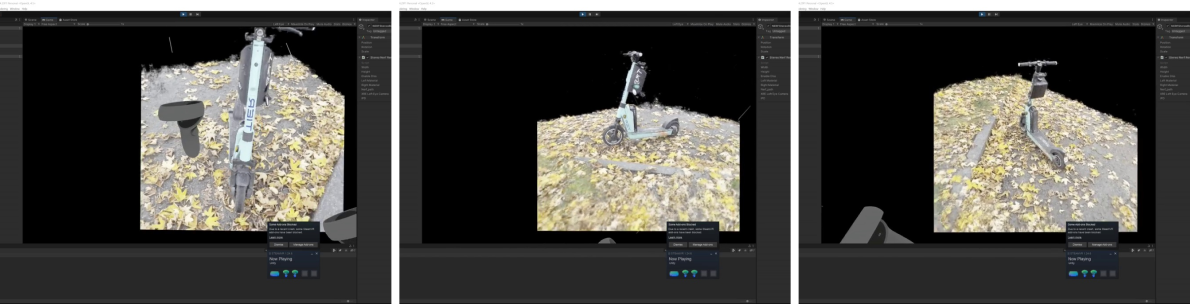
\includegraphics[width=\textwidth]{figures/tier_vr.png}
    \caption{NeRF viewed in VR with the help of immersive-ngp \cite{immersive-ngp}}
    \label{fig:tier_vr}
\end{figure}


% From Discord thread
\begin{comment} 
\textbf{Wavy artifacts in Nerfacto:}
AFAIK those wavy artifacts are from how the nerfacto model does ray sampling. Sometimes for very thin objects, none of the samples across a ray will land on it, causing it not to be visible in the rendering 

\textbf{Better results with another model?}
One of the reasons nerfacto is so fast is because it learns the distribution of weight across a ray, then samples from that distribution to get the ray samples. This means you aren't sampling where you don't need to, but also you might miss thin structures. Other methods might use more simple ray samplers that would densely sample across the ray, but would end up being a good bit slower to train/render
\end{comment}